\documentclass[tikz,crop]{standalone}

\usepackage{amsmath}
\usepackage{tikz}
\usepackage{siunitx}
\usetikzlibrary{arrows.meta,calc,shapes.geometric, positioning, patterns, patterns.meta}

\definecolor{frontpanel color}{RGB}{236, 228, 226}
\definecolor{power button}{RGB}{253, 245, 243}
\definecolor{front-rear button}{RGB}{231, 219, 219}
\definecolor{bumper}{RGB}{155, 146, 151}
\definecolor{secondary button}{RGB}{77, 131, 157}
\definecolor{secondary label}{RGB}{142, 159, 179}
\definecolor{function button color}{RGB}{245, 238, 236}
\definecolor{option button color}{RGB}{211, 202, 205}
\definecolor{copper}{RGB}{183,119,41}
\definecolor{aluminum}{RGB}{136,139,141}
\definecolor{styrodur}{RGB}{231,216,188}
\definecolor{fan color}{RGB}{230,210,186}
\definecolor{fan color dark}{RGB}{117,55,40}

\begin{document}
    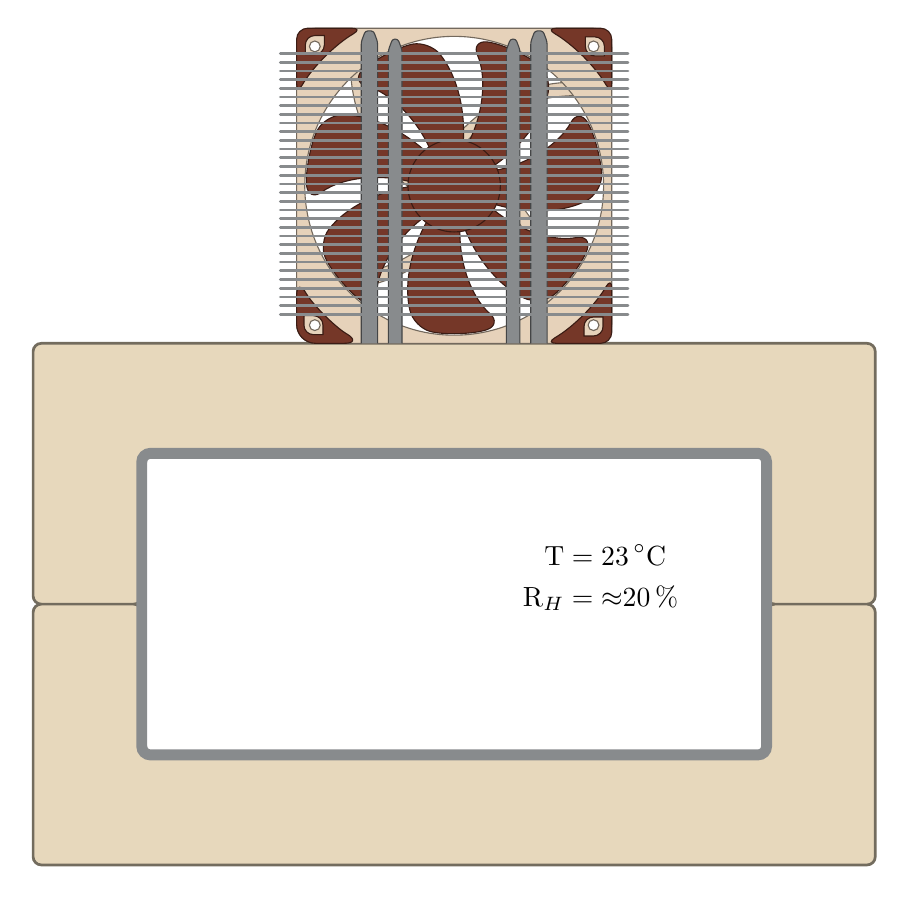
\begin{tikzpicture}
        % thermal chamber
        \begin{scope}[opacity=1]
            \def\sclThermal{.345}  %scaling factor of the thermal chamber symbol
            \coordinate (thermal chamber origin) at (0,0);
            \coordinate (box top left) at ($(thermal chamber origin) +(0,192mm*\sclThermal)$);
            \coordinate (box top right) at ($(thermal chamber origin) +(310mm*\sclThermal,192mm*\sclThermal)$);
            \draw[
                styrodur!50!black, fill=styrodur, line width=1mm*\sclThermal, rounded corners=3mm*\sclThermal
            ]
                (thermal chamber origin) -- ++(0,96mm*\sclThermal) -- ++(40mm*\sclThermal,0) -- ++(0,-56mm*\sclThermal) -- ++(230mm*\sclThermal,0) -- ++(0,56mm*\sclThermal) -- ++(40mm*\sclThermal,0) -- ++(0,-96mm*\sclThermal)  -- cycle
                (thermal chamber origin) ++(0,96mm*\sclThermal) -- ++(0,96mm*\sclThermal) -- ++(310mm*\sclThermal,0) -- ++(0,-96mm*\sclThermal) -- ++(-40mm*\sclThermal,0) -- ++(0,56mm*\sclThermal) -- ++(-230mm*\sclThermal,0) -- ++(0,-56mm*\sclThermal) -- cycle

            ;
            % aluminum box
            \draw[aluminum, rounded corners=9*\sclThermal, line width=4mm*\sclThermal]
                (thermal chamber origin) ++(40mm*\sclThermal,40.5mm*\sclThermal) -- ++(0,111mm*\sclThermal) -- ++(230mm*\sclThermal,0) coordinate(thermal top right) -- ++(0,-111mm*\sclThermal) -- cycle
            ;
            % cooler
            \begin{scope}
                % fan
                \coordinate(fan bottom left) at ($(box top left) +(97mm*\sclThermal,0)$);
                \coordinate(fan top right) at ($(fan bottom left) +(116mm*\sclThermal,116mm*\sclThermal)$);
                \coordinate(fan top left) at ($(fan bottom left) +(0,116mm*\sclThermal)$);
                \coordinate(fan bottom right) at ($(fan bottom left) +(116mm*\sclThermal,0)$);
                \coordinate(fan center) at ($(fan bottom left)!0.5!(fan top right)$);
                % fan body
                \draw[fan color!50!black, fill=fan color]
                    (fan center) ++(-10mm*\sclThermal,0) arc(160:90:58mm*\sclThermal) -- ++(0,-5mm*\sclThermal) arc(90:160:56mm*\sclThermal)
                    (fan center) ++(0,10mm*\sclThermal) arc(70:0:58mm*\sclThermal) -- ++(-5mm*\sclThermal,0) arc(0:70:56mm*\sclThermal)
                    (fan center) ++(10mm*\sclThermal,0) arc(340:270:58mm*\sclThermal) -- ++(0,5mm*\sclThermal) arc(270:340:56mm*\sclThermal)
                    (fan center) ++(0,-10mm*\sclThermal) arc(250:180:58mm*\sclThermal) -- ++(5mm*\sclThermal,0) arc(180:250:56mm*\sclThermal)
                ;
                \draw[fan color!50!black, fill=fan color, rounded corners=20*\sclThermal, opacity=1]
                     (fan bottom left)-- ++(0,116mm*\sclThermal) -- ++(116mm*\sclThermal,0) -- ++(0,-116mm*\sclThermal) -- cycle
                    (fan center) circle[radius=55mm*\sclThermal]
                    (fan bottom left) ++(6.7mm*\sclThermal,6.7mm*\sclThermal) circle[radius=2mm*\sclThermal]
                    (fan bottom right) ++(-6.7mm*\sclThermal,6.7mm*\sclThermal) circle[radius=2mm*\sclThermal]
                    (fan top left) ++(6.7mm*\sclThermal,-6.7mm*\sclThermal) circle[radius=2mm*\sclThermal]
                    (fan top right) ++(-6.7mm*\sclThermal,-6.7mm*\sclThermal) circle[radius=2mm*\sclThermal]

                ;
                % anti-vibration pads
                \draw[fan color dark!50!black, fill=fan color dark, rounded corners=7mm*\sclThermal]
                    (fan center) ($(fan center) + (210.04:67mm*\sclThermal)$) arc (210.04:239.96:67mm*\sclThermal) -- (fan bottom left) -- cycle
                    [sharp corners] (fan bottom left) ++(9.7mm*\sclThermal,6.7mm*\sclThermal) arc(0:90:3.5mm*\sclThermal) -- ++(-3.5mm*\sclThermal,0) -- ++(0, -3.5mm*\sclThermal) arc(180:270:3.5mm*\sclThermal) -- ++(3.5mm*\sclThermal,0) -- cycle
                    [rounded corners]
                    (fan center) ($(fan center) + (300.04:67mm*\sclThermal)$) arc (300.04:329.96:67mm*\sclThermal) -- (fan bottom right) -- cycle
                    [sharp corners] (fan bottom right) ++(-6.7mm*\sclThermal,9.7mm*\sclThermal) arc(90:180:3.5mm*\sclThermal) -- ++(0,-3.5mm*\sclThermal) -- ++(3.5mm*\sclThermal,0) arc(-90:0:3.5mm*\sclThermal) -- ++(0,3.5mm*\sclThermal) -- cycle
                    [rounded corners]
                    (fan center) ($(fan center) + (30.04:67mm*\sclThermal)$) arc (30.04:59.96:67mm*\sclThermal) -- (fan top right) -- cycle
                    [sharp corners] (fan top right) ++(-9.7mm*\sclThermal,-6.7mm*\sclThermal) arc(180:270:3.5mm*\sclThermal) -- ++(3.5mm*\sclThermal,0) -- ++(0,3.5mm*\sclThermal) arc(0:90:3.5mm*\sclThermal) -- ++(-3.5mm*\sclThermal,0) -- cycle
                    [rounded corners]
                    (fan center) ($(fan center) + (120.04:67mm*\sclThermal)$) arc (120.04:149.96:67mm*\sclThermal) -- (fan top left) -- cycle
                    [sharp corners] (fan top left) ++(6.7mm*\sclThermal,-9.7mm*\sclThermal) arc(270:360:3.5mm*\sclThermal) -- ++(0,3.5mm*\sclThermal) -- ++(-3.5mm*\sclThermal,0) arc(90:180:3.5mm*\sclThermal) -- ++(0,-3.5mm*\sclThermal) -- cycle
                ;
                % fan blades
                \begin{scope}
                    \foreach \i in {0,...,6} {
                        \draw[fan color dark!50!black, fill=fan color dark, rounded corners=6mm*\sclThermal]
                            (fan center) arc(237+\i*360/7:297+\i*360/7:54mm*\sclThermal) arc(-3+\i*360/7:32+\i*360/7:54mm*\sclThermal) arc(332+\i*360/7:272+\i*360/7:45mm*\sclThermal)
                        ;
                    }
                    \draw[fan color dark!50!black, fill=fan color dark] (fan center) circle[radius=17mm*\sclThermal];
                \end{scope}
                % heat pipes
                \begin{scope}
                    \draw[aluminum!50!black, fill=aluminum, rounded corners=0.9mm*\sclThermal]
                        (box top left) ++(120.8mm*\sclThermal,0) -- ++(0,111mm*\sclThermal) -- ++(1.5mm*\sclThermal,4mm*\sclThermal) -- ++(3mm*\sclThermal,0) -- ++(1.5mm*\sclThermal,-4mm*\sclThermal) -- ++(0,-111mm*\sclThermal)
                    ;
                    \draw[aluminum!50!black, fill=aluminum, rounded corners=0.9mm*\sclThermal]
                        (box top left) ++(130.8mm*\sclThermal,0) -- ++(0,108mm*\sclThermal) -- ++(1.5mm*\sclThermal,4mm*\sclThermal) -- ++(2mm*\sclThermal,0) -- ++(1.5mm*\sclThermal,-4mm*\sclThermal) -- ++(0,-108mm*\sclThermal)
                    ;
                    \draw[aluminum!50!black, fill=aluminum, rounded corners=0.9mm*\sclThermal]
                        (box top right) ++(-120.8mm*\sclThermal,0) -- ++(0,111mm*\sclThermal) -- ++(-1.5mm*\sclThermal,4mm*\sclThermal) -- ++(-3mm*\sclThermal,0) -- ++(-1.5mm*\sclThermal,-4mm*\sclThermal) -- ++(0,-111mm*\sclThermal)
                    ;
                    \draw[aluminum!50!black, fill=aluminum, rounded corners=0.9mm*\sclThermal]
                        (box top right) ++(-130.8mm*\sclThermal,0) -- ++(0,108mm*\sclThermal) -- ++(-1.5mm*\sclThermal,4mm*\sclThermal) -- ++(-2mm*\sclThermal,0) -- ++(-1.5mm*\sclThermal,-4mm*\sclThermal) -- ++(0,-108mm*\sclThermal)
                    ;
                    \foreach \y in {0,...,30} {
                        \draw[aluminum, line width=1mm*\sclThermal, line cap=round]
                            ($(box top left)+(91mm*\sclThermal,10.7mm*\sclThermal+\y*3.2mm*\sclThermal)$) -- ++(128mm*\sclThermal,0)
                        ;
                    }
                    \node[below left=of thermal top right, align=left]
                        {$\begin{aligned}
                            \text T &= \qty{23}{\celsius}\\
                            \text R_H &= \qty{\approx 20}{\percent}
                        \end{aligned}$}
                    ;
                \end{scope}
            \end{scope}
        \end{scope}
    \end{tikzpicture}
\end{document}
